% vim: set filetype=tex fileencoding=utf8 et sw=2 ts=2 sts=2 tw=80 :
% © 2014 Ali Polatel <polatel@gmail.com>
% Creative Commons Attribution-NonCommercial-ShareAlike 3.0 Unported Lisansı ile yayınlanmıştır.

\documentclass[12pt,a4paper,oneside,article]{memoir}
\setulmarginsandblock{3cm}{3cm}{*}
\setlrmarginsandblock{4cm}{2.5cm}{*}
\checkandfixthelayout
\fixpdflayout
\usepackage[T1]{fontenc}
\usepackage[turkish]{babel}

\usepackage{fontspec}
\defaultfontfeatures{Ligatures=TeX}
%\usepackage{unicode-math}
%\setmathfont[Script=Latin,Language=Turkish]{Tex Gyre Pagella Math}
\setmainfont[Script=Latin,Language=Turkish]{TeX Gyre Termes}
\setsansfont[Script=Latin,Language=Turkish]{TeX Gyre Termes}

\abstractintoc

\usepackage[round]{natbib}
\usepackage{babelbib}
\usepackage{tocbibind}
\bibliographystyle{plainnat}
\bibintoc

\cftinsertcode{toc}{\renewcommand*{\cftappendixname}{Ek \space}}
\renewcommand*{\appendixname}{Ek \space}
\renewcommand*{\appendixpagename}{Ekler}
\renewcommand*{\appendixtocname}{\appendixpagename}
\renewcommand*{\cftappendixname}{Ek \space}

\usepackage{graphicx}
\DeclareGraphicsExtensions{.jpg,.png}

\usepackage{multicol}
\usepackage{pdfpages}
\usepackage{indentfirst}
\usepackage[xspace]{ellipsis}

\pretitle{\begin{center}\vfill\Large\bfseries}
\title{Bilim Kurgu Çevirisi:\\All You Zombies, Robert A. Heinlein}
\posttitle{\par\end{center}\vspace{4em}}
\preauthor{\begin{center}\vfill}
\author{Al\.{}\kern-.3emi Polatel} % textsc{} & iİ conflict.
\postauthor{\\1101207005\par\end{center}}
\predate{\par\vfill\begin{center}}
\date{Edirne, 2014} % lazy.
\postdate{\par\end{center}}

\renewcommand{\maketitlehooka}{%
  \begin{center}
    T.C.\xspace\\
    Trakya Üniversitesi\xspace\\
    Edebiyat Fakültesi Mütercim Tercümanlık Bölümü\xspace\\
    İngilizce Mütercim Tercümanlık Ana Bilim Dalı\xspace\\
    Çeviri Projesi\xspace\\[1cm]

    \shorthandoff{=}
    
\includegraphics[width=2.5cm]{trakya}  % Üniversite logosu
    \shorthandon{=}
  \end{center}
}
\renewcommand{\maketitlehookc}{%
  \begin{center}
    \vspace{1em}
    \textbf{Danışman}\xspace\\
    Öğr. Gör. İnönü Korkmaz\xspace
  \end{center}
}

\newenvironment{dedication}
  {\clearpage           % we want a new page
   \thispagestyle{empty}% no header and footer
   \addcontentsline{toc}{chapter}{İthaf} % Add to TOC
   \vspace*{\stretch{1}}% some space at the top 
   \centering           % 
  }
  {\par % end the paragraph
   \vspace{\stretch{3}} % space at bottom is three times that at the top
   \clearpage           % finish off the page
  }

\usepackage[unicode]{hyperref}
\hypersetup{%
    hyperfootnotes=true,
    breaklinks=true,
    colorlinks=true,
    urlcolor=black,
    citecolor=black,
    linkcolor=black,
    pdftitle={Bilim Kurgu Çevirisi: ``All You Zombies'', Robert Heinlein},
    pdfauthor={Ali Polatel},
    pdfsubject={Ali Polatel, Lisans Bitirme Ödevi, Çeviri Projesi},
    pdflang={tr},
    pdfkeywords={robert heinlein, çeviri, bilim kurgu, bilim kurgu çevirisi, erek metin odaklı çeviri},
    pdfproducer={LuaLaTeX, BibTeX, hyperref, memoir},
    pdfpagelabels=true
    pdfborder={0 0 0},
}
\pdfcompresslevel=9

\begin{document}

\OnehalfSpacing

\calccentering{\unitlength}
\begin{adjustwidth*}{\unitlength}{-\unitlength}
  \begin{adjustwidth}{-1cm}{-1cm}
    \begin{titlingpage}
      \maketitle
    \end{titlingpage}
  \end{adjustwidth}
\end{adjustwidth*}

\frontmatter

% vim: set filetype=tex fileencoding=utf8 et sw=2 ts=2 sts=2 tw=80 :
% © 2014 Ali Polatel <polatel@gmail.com>
% Creative Commons Attribution-NonCommercial-ShareAlike 3.0 Unported Lisansı ile yayınlanmıştır.

\thispagestyle{empty}
\chapter*{Önsöz}
\addcontentsline{toc}{chapter}{Önsöz}

2013-2014 öğretim yılı bahar dönemi \textbf{Çeviri Projesi} dersi için hazırlamış
olduğum bu belge, ABD'li bilim kurgu yazarı \textsc{Robert A.  Heinlein}
(1907-1988) tarafından kaleme alınan ve ilk olarak \emph{The Magazine of
Fantasy and Science Fiction} dergisinin 1959 yılı Mart sayısında yayınlanmış
olan \emph{``All You Zombies--''} adlı kısa hikayenin asıl metni ve çevirisiyle
beraber bu çeviriyi yaparken karşılaştığım sorunlar ve izlediğim yöntemlerin bir
özetini içermektedir.

Belge, \LaTeX ve \textsc{Bib}\negthinspace\TeX\hspace{1pt} kullanılarak baskıya hazırlanmıştır.

\begin{flushright}
  \textsc{\theauthor}\\
  Edirne, Mayıs 2014
\end{flushright}


% vim: set filetype=tex fileencoding=utf8 et sw=2 ts=2 sts=2 tw=80 :
% © 2014 Ali Polatel <polatel@gmail.com>
% Creative Commons Attribution-NonCommercial-ShareAlike 3.0 Unported Lisansı ile yayınlanmıştır.

\calccentering{\unitlength}
\begin{dedication}
  \begin{adjustwidth*}{\unitlength}{-\unitlength}
    \begin{adjustwidth}{-1cm}{-1cm}
      \hspace{4cm}
      \emph{Rüyalarıma hükmeden güzel Nünü'ye}
    \end{adjustwidth}
  \end{adjustwidth*}
\end{dedication}


% vim: set filetype=tex fileencoding=utf8 et sw=2 ts=2 sts=2 tw=80 :
% © 2014 Ali Polatel <polatel@gmail.com>
% Creative Commons Attribution-NonCommercial-ShareAlike 3.0 Unported Lisansı ile yayınlanmıştır.

\thispagestyle{empty}
\chapter*{Teşekkür}
\addcontentsline{toc}{chapter}{Teşekkür}

Öğretmenlerim \textsc{Dolunay Kumlu}'ya ve \textsc{İnönü Korkmaz}'a,

Sırdaşım \textsc{Mer\.{}\kern-.3emiç} \textsc{Nehr\.{}\kern-.3emi}'ne,

Divane elmas \textsc{Roger Keith Barrett}'a

Vefalı dostum \textsc{T.T. Hüsey\.{}\kern-.3emin Kara}'ya,

\vspace{.5cm}

İçtenlikle teşekkür ederim. İyi ki varsınız.


\tableofcontents

\mainmatter
\pagestyle{simple}
\chapterstyle{ntglike}

% vim: set filetype=tex fileencoding=utf8 et sw=2 ts=2 sts=2 tw=80 :
% © 2014 Ali Polatel <polatel@gmail.com>
% Creative Commons Attribution-NonCommercial-ShareAlike 3.0 Unported Lisansı ile yayınlanmıştır.

\chapter{Bilim Kurgu ve Bilim Kurgu Çevirisi Üzerine}

Bilim kurgu, temelini bilimsel ve teknolojik unsurlardan alsa da yarattığı
kurgusal evreninde fiziki ve doğal evrenin sınırlarının yerini hayal gücünün
sınırları alır. Bu bağlamda tanımlanması güçtür ve geniş, belirsiz sınırlarının
içinde birçok alt tür barındırmaktadır.

Döneminin en başarılı bilim kurgu yazarlarından biri olarak kabul edilen ve
adından sıklıkla ``bilim kurgu yazarlarının duayeni'' \citep{SFH09}
olarak söz ettiren \textsc{Robert A. Heinlein}'ın (1907--1988) yaptığı bilim
kurgu tanımı, türün genel hatlarını betimlemektedir: ``Neredeyse bütün bilim
kurguyu kapsayan kullanışlı, kısa bir tanım şöyle olabilir: Temelini gerçek
dünya, geçmiş ve şimdiki zaman hakkında yeterli bilgi ve doğa ile bilimsel
yöntemlerin kapsamlı bir anlayışı üzerine sağlam olarak oturtan, gelecekteki
olası olaylar üzerine yapılan gerçekçi kurgulamalar.'' \citep{SFN59}
Dilimizdeki \emph{bilim kurgu} ifadesinin \emph{isim
babası} olan yazar ve gazeteci \textsc{Orhan Duru} (1933--2009) da bilim kurguyu
benzer şekilde tanımlamıştır: ``Bilim-Kurgu'yu tanımlamak çok zor. Kişinin ve
yazarın görüşüne göre değişiyor.  Bu tanım, gerçeklerle, bilimsel verilerle bir
ölçüde sınırlı bir düşçülük diyebiliriz bilim-kurguya.'' \citep{XBil76}

Bilim ve bilimin \emph{omuzlarında yükselen} bilim kurgu arasındaki etkileşim,
yazın türünün doğuşundan bugüne kadar süregelmiştir. \textsc{Schwartz}, \emph{Bilim
Kurgu: İki Kültür Arasındaki Köprü} yazısında bu ilişkiyi örneklendirerek
açıklar: ``Bilim ve kurgu arasında iki yönlü sürekli bir etkileşim vardır,
örneğin \emph{Ray Bradbury: Story of a Writer (Sterling)} filminde yazarın yeni
kısa hikayesi için gerekli bilgiyi elde etmek üzere bir telefon bilgisayar
merkezine gittiğini görürüz. Düzyazı geleneğimizde ilk defa baskın hale gelen bu
emsalsiz ilişkiden ötürü bilim kurgu çağımızı en iyi yansıtan edebi tür olarak
görülebilir.'' \citep{schwartz71}

Günümüzden geriye bakıldığında bilim kurgunun bilim için bir esin kaynağı, bir
tetikleyici güç olduğu görüşü gitgide daha fazla benimsenmektedir. Teorik
fizikçi \textsc{Michio Kaku} bu durumdan coşkuyla söz eder: ``Sicim teorisi
gibi gelişmiş teorilerin ortaya çıkmasıyla birlikte zaman yolculuğu ve paralel
evrenler gibi yalnızca bilim kurguya ait olan kavramlar dahi artık fizikçiler
tarafından yeniden değerlendiriliyor. Yüz elli sene önce zamanın bilim insanları
tarafından `imkansız' olarak nitelenen ve şimdi günlük hayatımızın birer
parçası olan teknolojik gelişimleri bir düşünün. Jules Verne'in 1865 yılında
yazdığı \emph{Yirminci Yüzyılda Paris} adlı kitap bir yüzyıldan fazla bir süre
sonra torununun oğlu tarafından tesadüfen bulunana ve 1994 yılında ilk kez
basılana dek saklı kalmıştı. Verne, kitapta Paris'in 1960 yılında nasıl
görüneceğini tasvir ediyordu. Romanı on dokuzuncu yüzyılda açıkça imkansız
olduğu ifade edilen teknolojilerle doluydu: Faks makineleri, dünya çapındaki bir
iletişim ağı, cam gökdelenler, doğalgazlı arabalar, yüksek hızlı trenler.''
\citep{PhyIMP09}

Bilim kurgu, yaratıcı ve üretken yapısıyla yazıldığı dillere de katkı yapmakta,
yeni kelime ve deyişlerin türetilmesinin öncüsü olmaktadır. Örnek olarak
İngilizce diline \textsc{Robert A. Heinlein} tarafından kazandırılan
\emph{``grok''} kelimesi gösterilebilir. \textsc{Stranger in a Strange Land}
adlı kitabın birçok yerinde geçen kelimenin yine aynı kitap içinde tanımı da
verilmiştir: ```Grok' o denli derinlemesine kavrayıştır ki gözlemci, gözlenenin
bir parçası olur: Birleşir, uyum sağlar, birbirleriyle evlenirler ve kimlikleri
birliklerinin içinde kaybolur. Din, felsefe ve bilim derken aklımıza gelenlerin
neredeyse hepsidir -- ve bize ifade ettiği anlamın, renklerin kör bir adam için
ifade ettiği anlamdan bir farkı yoktur.'' \citep{SSL61} Kelime, başta okur
kitlesi sonrasında da toplum tarafından kabul görmüş, kullanılmaya başlanmış ve
sözlüklerde yerini almıştır. Kelimenin \emph{Oxford Dictionary of English}
sözlüğündeki tanımı: ``(bir şeyi) sezgiyle veya empatiyle anlamak''tır
\citep{Oxford05}.

Çeviribilim çerçevesinde bilim kurgu incelenecek olursa hali hazırda
tanımlanması zor olan kaynak metnin erek dil ve kültür çerçevesinde işlev ve
amacının belirlenmesi gerekecektir. Bu açıdan ortaya çıkacak sorunlar genel
olarak bakıldığında teknik çevirilerde \citep{Aksoy1998} ve edebi çevirilerde
karşılaşılan sorunların \citep{BengiÖner1999} bir harmanı şeklindedir. Çevirmen,
bir yandan kurgunun temelinde var olan teknik alt yapıyı diğer yandan da eserin
edebi havasını erek dile taşımak durumundadır. Kaynak metnin derinlemesine
analiz edilmesi, çeviri metninin erek dildeki işlevi ve amacının belirlenmesiyle
birlikte çeviri için bir plan ve yöntem seçilmesi asıl çeviri işlemine
başlamadan önce yapılmalıdır.

\textsc{Robert A. Heinlein}'ın ``All You Zombies--'' adlı kısa hikayesi, günlük
bir dilde yazılmıştır ve özellikle giriş bölümünde sık olarak argo kullanımına
başvurulmuştur. Yazar bu anlatım şekliyle okuyucusunu içinde bulunduğu dünyadan
yavaşça hikayenin içine çeker. Ardından da \emph{zaman yolculuğunun} çelişkili
doğası adım adım okuru sarar. Teknik alt yapı olarak neredeyse hiçbir art-alan
bilgisi öngörmez. Yazar okurun ihtiyacı olan bütün bilgiyi - kimi zaman açık
bir dille, kimi zaman da üstü kapalı olarak \emph{satır aralarında} -
vermektedir. \textsc{H.G. Wells}'in 1895 yılında yazdığı bu alt türün öncüsü
kabul edilen ``Zaman Makinesi'' romanının aksine ``All You Zombies--''
hikayesindeki anlatım şekli yazı boyunca aynı kalmaz. Yazarın yaptığı hızlı
değişiklikler akıcılığı körüklemekte, \emph{zaman yolculuğunun} fiziksel
imkansızlıkları ve felsefik çapraşıklıklarını \emph{sıradan} bir dünyada yaşayan
okurun yüzüne vurmaktadır.

Kaynak metin ile ilgili yapılan bu analiz ve ilgili kabuller ışığında çeviri
için yöntemler belirlenmiştir. Çevirmenin öncelikli amacı bahsi geçen bu kafa
karıştırıcı mizahı erek dile taşımaktır. Yazarın \emph{üstü kapalı} kalmasını
yeğlediği detaylar için erek metinde herhangi bir ek açıklama yapılmayacaktır.

\include{çeviri}
% vim: set filetype=tex fileencoding=utf8 et sw=2 ts=2 sts=2 tw=80 :
% © 2014 Ali Polatel <polatel@gmail.com>
% Creative Commons Attribution-NonCommercial-ShareAlike 3.0 Unported Lisansı ile yayınlanmıştır.

\chapter{Çevirinin Değerlendirilmesi}

Çeviri öncesinde yapılan kabullere göre, çeviri süreci boyunca düz ve
yananlamsal eşdeğerlilik ile beraber dil-kullanımsal ve biçimsel eşdeğerliliğin
de (kavramlar için \citealp[bkz.][]{GokturkEsdeger}) sağlanmasına çabalanmıştır.
Kaynak metne bağlılık ise hikayenin değişken doğası sebebiyle her noktada aynı
ölçüde değildir.

Çeviriyi yaparken yukarıda bahsi geçen eşdeğerlilikleri sağlamak adına belli
noktalarda ifadeler erek dile uyarlanmış, diğer noktalarda ise buna gerek
görülmemiştir. Bu iki duruma birer örnek aşağıda verilmiştir.

\begin{enumerate}
  \item
    Kaynak metinde ana kahramanın katılmayı planladığı \emph{W.E.N.C.H.} adlı kurum,
    farklı dönemlerde \emph{A.N.G.E.L.} ve \emph{W.H.O.R.E.} şeklinde de anılmıştır.
    Son kısaltma metinde direkt olarak belirtilmemiş fakat ilk iki kısaltmanın
    açılımlarına değinildikten sonra kurumun \emph{üçüncü bir ismi} de olduğu ifade
    edilerek açılımı verilmiştir: \emph{Women's Hospitality Order Refortifying \&
    Encouraging Spacemen}. İngiliz dilinde \emph{backronym} olarak adlandırılan bu
    kelime oyunu, ``var olan bir kısaltma veya kelimenin gerçek kullanımına
    dayanmayan şekilde açılmasıdır'' \citep{OxfordBackronym}.

    Bu tür kısaltma açmalarına İngiliz dilinden verilebilecek uygun bir örnek
    \emph{Erasmus Programı}'ndaki \emph{Erasmus} kelimesinin kullanımıdır. Özel bir
    isim olan Erasmus kelimesi, adını kullanan programın amacını da belirtmesi için
    ``European Community Action Scheme for the Mobility of University Students''
    şeklinde açılmıştır \citep{WkErasmus}. Dilimizde \emph{kin} kelimesinin
    ``kişinin içindeki nefret'' \citep{SesliBackronym} olarak açılması da benzer bir
    durumdur.

    Kısaltmaların dipnot ile açıklanması çevirinin yeterliliğiyle ilgili iki
    sorun oluşturmaktadır:

    \begin{enumerate}
      \item
        Hikayede kısaltmalar birden fazla yerde geçmektedir. Dolayısıyla dipnot ile
        açıklama erek dildeki okur için hikayenin akıcılığını zedeler.
      \item
        Yazar üçüncü kısaltmanın yalnızca açılımını vermiş, baş harflerinden bir
        kelime oluşturup oluşturmamayı okura bırakmıştır. Dolayısıyla verilecek
        dipnot yazarın bu \emph{üstü kapalı} biçeminin erek dil okuruna
        yansıtılmasını engeller.
    \end{enumerate}

    Bu sebeplerden ötürü kısaltmaları uyarlama yoluna gidilmiştir. Kısaltmalardan
    ikisinin kaynak dilin argosuna ait oluşu da göz önünde bulundurulmuştur.
  \item
    Kaynak metinde geçen \emph{servis station} ifadesi üzerine birden fazla
    anlam yüklenen bir diğer kullanımdır. Yazar, hikayenin iki farklı dönem
    (Churchil dönemi ve anlatıcının şimdiki zamanı) için bu ifadeye birbirinden
    bütünüyle farklı iki anlam yüklemektedir. Ancak bu iki anlamın da
    Güttinger'in ortaya koyduğu şekilde ``kaynak ve erek dillerde aynı etkiyi
    yaratması'' \citep{GokturkEsdeger} için ``kelimesi kelimesine çeviri''
    \citep{NewmarkTextbook} ile erek dile aktarımı eşdeğerliliği sağlayabilir:
    \emph{(akaryakıt) servis istasyonu} ifadesi erek dilde kullanılmaktadır.
    Kelimeye yüklenen diğer anlamın da, kaynak dildeki \emph{escort
    agency/service} ifadesinin erek dile \emph{eskort servis} olarak taşınmış
    olduğu dikkate alındığında, en azından benzer bir etki yaratacağı açıktır.
\end{enumerate}

Bilim kurguya özgü olan ve/veya yazar tarafından türetilmiş ifadeler anlamları
koruyacak şekilde taşınmaya çalışılmıştır. Bunun mümkün olmadığı bir durumda -
hikayede \emph{Old Underwear} adıyla anılan içki örneğinde - erek dilde benzer
bir anlatımı yakalamak üzere yeni bir ifade türetilmiştir: \emph{Don Murdar}.

\aliaspagestyle{part}{simple}
\appendix
\appendixpage
\addappheadtotoc
\aliaspagestyle{part}{}
% vim: set filetype=tex fileencoding=utf8 et sw=2 ts=2 sts=2 tw=80 :
% © 2014 Ali Polatel <polatel@gmail.com>
% Creative Commons Attribution-NonCommercial-ShareAlike 3.0 Unported Lisansı ile yayınlanmıştır.

\chapter{Kaynak Metin: ``All You Zombies--''}
\chapterprecis{The Magazine of Fantasy and Science Fiction, Mart 1959}

\begin{center}
  \shorthandoff{=}
  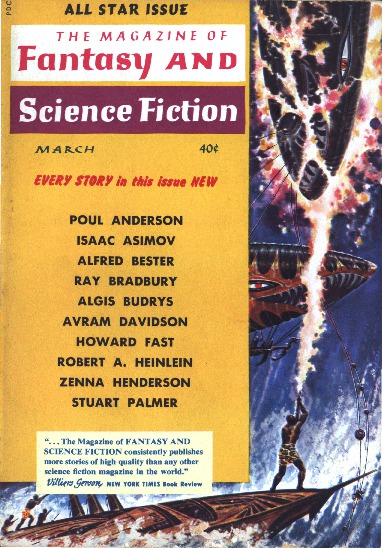
\includegraphics[width=12em,keepaspectratio]{scifi59}
  \shorthandon{=}
  \\
  \shorthandoff{=}
  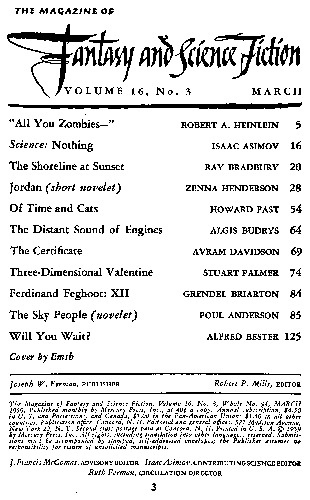
\includegraphics[width=13em,keepaspectratio]{scifi59-index}
  \shorthandon{=}
\end{center}

\shorthandoff{=}
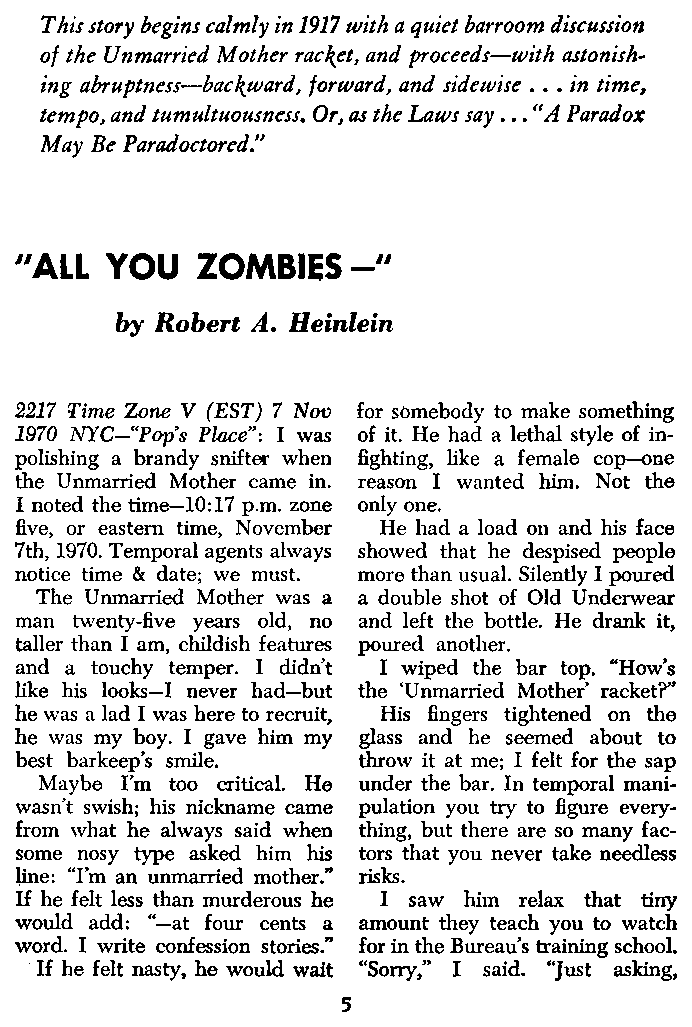
\includepdf[pages=-]{zomby.pdf}
\shorthandon{=}


\backmatter
% vim: set filetype=tex fileencoding=utf8 et sw=2 ts=2 sts=2 tw=80 :
% © 2014 Ali Polatel <polatel@gmail.com>
% Creative Commons Attribution-NonCommercial-ShareAlike 3.0 Unported Lisansı ile yayınlanmıştır.

\thispagestyle{empty}
\chapter*{Sonsöz}
\addcontentsline{toc}{chapter}{Sonsöz}

\textbf{Çeviri Projesi} dersi için bilim kurgu çevirisini ve bu çeviri sırasında
yaşadığım sorunları inceledim ve bunlara çözüm önerileri getirmeye çalıştım.

Hamurunda yaratıcılık olan bilim kurgu ile amacı anlamı taşımak olan işlevsel,
amaca yönelik çevirinin birbirini tamamlar nitelikte olduğu fikrindeyim. Bu
yazın türündeki eserlerin erek dile kazandırılmasının bu dile yeni bir eser
kazandırmanın ötesinde kaynak dil okurunda uyandırdığı merağı ve keşfetme
arzusunu erek dil okurunda da uyandırdığını düşünüyorum.

\begin{flushright}
  \textsc{\theauthor}\\
  Edirne, Mayıs 2014
\end{flushright}

\bibliography{Heinlein-All-You-Zombies-tr-alip}

\end{document}
